\FloatBarrier

\begin{figure}[htbp]
\centering
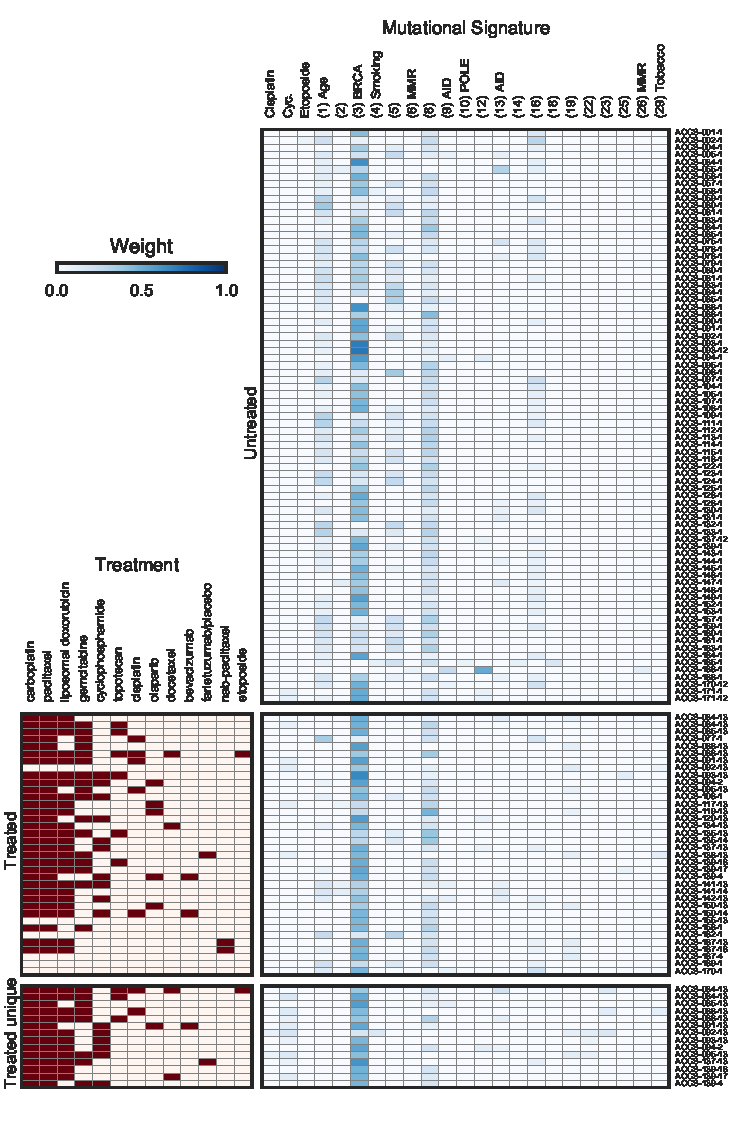
\includegraphics[scale=1.0]{figures/signatures.pdf}
\caption{\textbf{Detected mutational signatures for donor-matched primary/untreated and relapse/treated samples.} \textit{(Top)} Signatures detected in the pre-treatment samples. The first four signatures were extracted from reports of a \textit{G. gallus} cell line and \textit{C. Elegans} after exposure to chemotherapy, and the rest are COSMIC curated signatures. COSMIC signature numbers are shown in parentheses, and the associated mutagenic process is indicated when known. Signatures not shown were undetected in these samples. \textit{(Bottom)} Clinical treatments and detected signatures for the mutations unique to the post-treatment samples (those with no evidence in the matched pre-treatment sample). Cases where a chemotherapy signature is detected are annotated with a (*) if the patient received the associated drug and a (?) otherwise.}
\label{fig:signatures}
\end{figure}

\begin{figure}
\centering
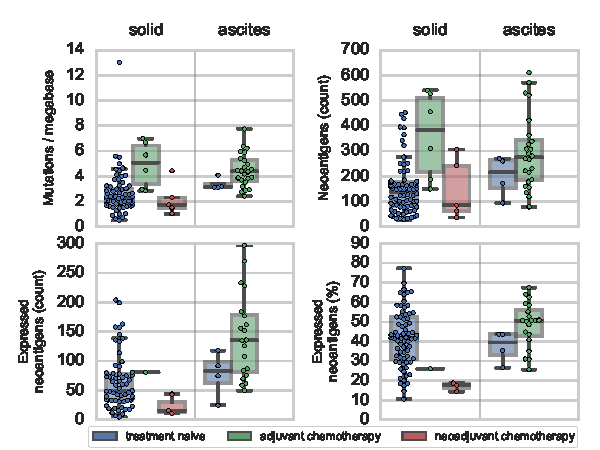
\includegraphics[scale=1.0]{figures/counts.pdf}
\caption{\textbf{Stratified comparison of mutation and neoantigen burden of chemotherapy-treated and untreated samples.} Mutations (upper left), neoantigens (upper right), and expressed neoantigens by count (lower left) and as a percent of total neoantigens (lower right) are shown for primary/untreated samples (blue; solid tumor n=75, ascites n=4), primary/treated samples (green; solid tumor n=5), and relapse/treated samples (red; solid tumor n=6, ascites n=24). The shaded boxes indicate the interquartile region and the median line. Points indicate individual samples.}
\label{fig:counts}
\end{figure}

\begin{figure}[htbp]
\centering
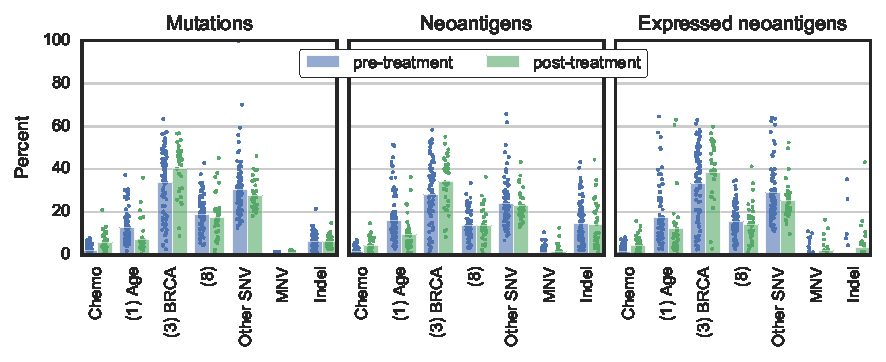
\includegraphics[scale=1.0]{figures/sources_of_mutations_and_neoantigens.pdf}
\caption{\textbf{Contribution of key SNV signatures, MNVs, and indels on mutations \textit{(left)}, neoantigens \textit{(center)}, and expressed neoantigens \textit{(right)}.} The \textit{Chemo} category combines the contributions from the chemotherapy signatures (cisplatin, cyclophosphamide, and etoposide). COSMIC signature numbers are in parentheses. The \textit{Other SNV} category represents SNVs not accounted for by the signatures shown. Bars give the mean, and points indicate individual samples.}
\label{fig:sources}
\end{figure}

\FloatBarrier
